\section{Domain Interpretation}
\label{sec:interpretation}
After we compute the probabilities from the classification section, we need to produce a final interpretation of the graph in terms of edges, vertices, arrows, self-loops, connections between edges and vertices and connections between arrows and edges. To do this we cannot use the trivial method of partitioning the graph into segments (from our segmentation step) and simply solving for the partition that produces the largest sum of classification probabilities (from the classification step). This is mainly because there is significant interaction between components of a graph. The design that we follow rests on the idea that the connections between the components influence the selection of the best interpretation.\\

\subsection{Scoring Subgraphs}

We found it useful to rank candidate graphs by scores that are formed from a range of metrics like sum of classifier probabilities $g(p)$, total number of components $C(p)$, number of connections $D(p)$ and number of missing connections $M(p)$. Thus, the combined score is simply: $V_{A,B,C}(p) = g(p) + A.C(p) + B.D(p) + C.M(p)$ where $g(p) = \sum_{(a_i,b_i,c_i) \in p}f(a_i, b_i, t_i)$. The function $f$ is determined by the classification probabilities. The score however is 0 when any component in $p$ has a probability less than 0.2. To properly assess the connections, we had to establish a set of machine specifications for our components where we could find the distances, say, between an edge and vertex or an edge an arrow.\\

Write machine specification.The recognition step provided some unique challenges. Here, an exhaustive search for candidate graphs had to be done because in the classification step we returned probabilities of all possible components. Since there are four different components that we consider: arrow, edge, vertex, loop, any segment can be one of the four components. Hence, the total number of candidate graphs to be considered at any step in the online setting is $4^{n_{segments}}$. We obtain $n_{segments}$ from the segmentation step where segmentation points are calculated from strokes. For each segment once classification is done, we first create a Cartesian product of components to include all possible combinations. Then each combination is converted to conform with our machine specifications (please refer to interpretation.py in our code). Next each combination (also a subgraph) is added to the locked-in graph to form the subgraph at step $i$. The score function assesses each such subgraph and assigns a final score. This final score is calculated using the connections formed between components in the classified graph and using the sum of probabilities acquired from the classification step. We discard the sum of probabilities for any subgraph if any of its components had less than 0.2 probability. This essentially means we filter out the subgraphs with extremely unlikely components. *Equation of score* The candidate subgraphs are sorted in descending order of their final scores. The highest scoring subgraph is treated as the interpreted graph for that step. Subsequently, the interpreted graph becomes the locked-in graph for the next step of handling user strokes and the pipeline is run again to find the interpreted graph at the end of the step.\\

In addition to the classification probability, the scoring depends on the connections too. Since the number of components tend to be over-counted by this method, it has a negative coefficient. The number of connections made has a positive coefficient because ideally, we want our interpretation module to detect as many connections as possible. A slightly more complex metric is the number of missing connections. To calculate it, we must penalize the graphs for having edge points not connected to vertices, arrows not connected to edges and self-loop with different starting and end vertices. The penalty is ensured here again by a negative coefficient. Finding loops connected to different vertices was challenging as looking for the same loop in two different connections was not an easy task. We resolved this by doing an element-wise comparison of the loop points.\\

\subsection{Connections}

A vertex-edge connection is tested for every vertex and edge pair. We can use the center and radius of the vertex to find the distance from the endpoints of the edge as edges are given as a set of target points that represent a smooth line. Computing the Euclidean distance between the center and each of the two endpoints of the edges gives us an idea of whether the connection is plausible. Of course, we must subtract the radius of the circle itself and threshold the resulting distance to discard the large distance values. We maintain a score q for each edge end point that is initialized to infinity and updated if and only if a new vertex is found for the end point such that it's distance falls below the threshold and it is less than the previous q (negative values are clipped to 0).\\

The arrow-edge connection algorithm is more complex because it involves triangles (machine specification for arrows) and lines (edges) that must intersect one of the sides of the triangle. Again, connection is tested for every arrow and edge pair (from the endpoints of the edge). Here, we first extend the edge sequence by adding a target point before the end point such that smoothness is still maintained (use the slope for this). The distance between the new and the old point is $\gamma$ . Now, we test for the segment between each consecutive pair of the extended edge. If the segment intersects with a side of the triangle, then two conditions must be satisfied. The first is that the distance between the endpoint and the point of intersection must be under the threshold or the distance between the endpoint and the point opposite to the intersection side of the triangle must be under the threshold. The second condition is valid only for arrows that were initially two-sided. It states that the side involved in the intersection is the same as the one that was initially non-represented by the user's drawing.\\

The central portion of domain interpretation is calculating the vertex-edge and arrow-edge connections. The vertex-edge calculation was relatively simple since the center is provided by the classification module. The next steps involve comparing the distances between the edge endpoints and the center of the circle. Based on a threshold, it is determined whether the edge end point is close enough to the vertex to form a connection. Since an endpoint can be connected to at most one vertex, we iteratively update the connection and finally end up pairing the edge with the vertex that has the minimum distance to the circumference of the vertex (or circle). Constructing an algorithm for arrow-edge connections was much more difficult. Since an arrow is represented with a triangle, choosing the correct orientation of the triangle is very important. Finding the intersection point of the edge and a side of the triangle helps in getting the correct orientation. Adding an extra point after the original endpoint made sense as it brought the edge closer to the correct corner of the arrow. This made it easier to do a threshold-based check on the distance between the new endpoint and the correct corner or the new endpoint and the midpoint of the intersecting side to determine the validity of the connection. Here also we have the constraint of an arrow being able to connect to at most one edge endpoint. The new endpoint was added utilizing the nearby slope of the edge as follows: * Equation of new point using slope*

\subsection{Cost Calculation}

We followed algorithm 1 in (cite) to calculate the cost of a hand-drawn graph's interpretation using our algorithm. The cost is nothing but the number of subgraphs the algorithm gets wrong. This means that the lower the cost, the better the performance. When we say subgraph, we mean the subgraph obtained after adding the strokes inputted in step $i$ to the subgraph that was locked-in at step $i-1$. The concept of a locked-in graph is important in an online setting as this means that the subgraph that has already been interpreted cannot be changed. This follows from the online goal of analyzing the graph at most five components at a time. A fundamental struggle in this step was to come up with a good function to check whether the interpreted subgraph is isomorphic to the intended subgraph as required by the algorithm. Since it is not tractable to try all permutations of vertices, we opted to focus on a few well-known heuristics. Checking for the number of vertices and edges and the vertex degree sequences of both the graphs often works well for simple graphs. We used just these three conditions to detect isomorphisms. Other heuristics like checking whether the degrees of adjacent vertices match were complex and hence we did not try them. We also checked isomorphisms only for the undirected versions of directed graphs as it was very unlikely in our case that directed graphs are isomorphic, but their undirected versions are not.\\

Training is done by post-processing the sketches of users. Since we are implementing the online method now, our recognition is triggered a fixed time after the user stops sketching. We do not want the already graph to change. Hence, the "locked-in" portion of the graph doesn't change here. New connections are made between the newly drawn components and the locked in components by a recognizer. The recognizer maintains a sequence of added strokes and the corresponding sub-graphs. For every pair, we select the most promising candidate graph according to our scores. However, if an isomorph exists, we select the isomorph as the representation of the intermediate subgraph. If there exists no isomorphism, then we penalize all the remaining pairs of new strokes and subgraphs.\\

After successfully completing the online method, we will work on the offline method. There are some fundamentally different aspects to the offline method like the recognizer will only act on the graph after completion and connections do not have to maintained to a locked-in graph. We aim to have an effective offline interpretation as our ambitious goal.\\

\subsection{Experiments and Results}

\begin{table}[!htb] %% use b,t,h
    \centering
    % you can use l,r,c for left-aligned, right-aligned or centered columns
    \begin{tabular}{lrr}
    \toprule
       Graph & Avg. Cost & Steps \\ % use ampersands to separate columns and \\ for end of rows
         \midrule
3  & 2.4 & 3  \\ 
4 & 2.0 & 3 \\
6 & 1.6 & 2 \\
7 & 2.8 & 3 \\
9 & 2.6 & 3 \\
11 & 3.6 & 4 \\
13 & 5.6 & 6 \\
         \bottomrule
    \end{tabular}
    \caption{Average cost of interpreting 7 graphs with 5 trials each}
    \label{tab:table_cost}
\end{table}

We conducted our experiments using the end-to-end pipeline (shown in the IPython notebooks in the repository) of segmentation, classification, and interpretation for each step, where a step signifies a set of user strokes that are analyzed by this pipeline and added to the locked-in graph to form a new locked-in graph. We selected graphs 2,3,4,6, 7, 11 and 13 from the mechanical turk experiment 1 as listed in the (cite). Each graph was drawn five times with five components added in each step, except the last step where five or less components were added. The five components being added in a particular step of a graph were not the same across trials, i.e., we didn't always add the same five components for step 1 of graph 7. Table shows the average cost of interpreting each graph. Naturally, the average cost is going to be more for graphs that require more steps to be drawn. Hence, the average total cost does not particularly help in comparing the algorithm's performance across graphs. Hence, we constructed a plot in figure which shows the average cost of steps 1 and 2 for all the graphs. Since not incurring cost at step $i$ requires the cost at step $i-1$ to be 0, the average cost for step 2 will always be more than or equal to the average cost of step 1 for a particular graph. We also trained within the parameter space stated in (cite) to obtain the best coefficients of the terms used in the candidate subgraph scoring function. Several combinations yielded the lowest cost including A = -1.1, B = 0.3 and C = -0.4.

\begin{figure}[!htb]
    \centering
    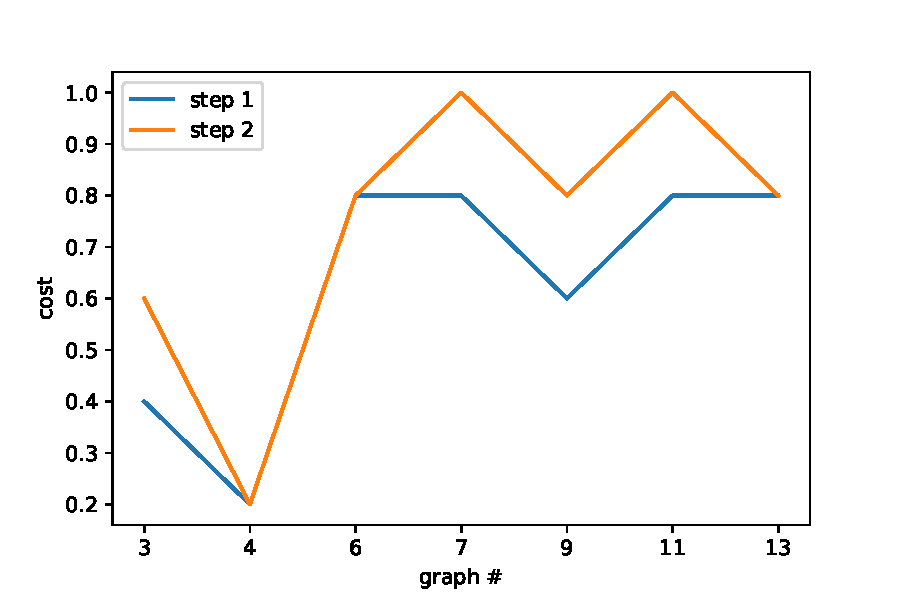
\includegraphics[scale=0.55]{./img/cost_plot.pdf}
    \caption{average cost of step 1 and step 2 for the 7 graphs}
    \label{fig:cost_plot}
\end{figure}

\subsection{Analysis}

The table shows that our pipeline did not perform exceptionally well. This was mainly because the cost, as defined in \cite{daly2015hand}, is a very harsh penalty. It is binary with no partial reward for some or most of the subgraph being correct. Since the correctness of an interpreted subgraph is determined by whether it is isomorphic to the intended subgraph, the cost at a particular step will 0 if and only if there is an isomorphism between the two. Other issues that affect our algorithm is the fact that we reuse the thresholds from (cite). These thresholds may not be appropriate for our drawing setting in iPyCanvas \cite{ipycanvas}. Training for finding our own values for the coefficients in the scoring step was not very helpful. A reason could be the search space for the parameter grid search was not right. Another potential weakness is probably the inconclusive isomorphism function. Figure shows that subgraphs with vertex and edges are more easily interpreted than those with loops and arrows. This was expected as circles for vertices and smooth lines for edges are much easier to break into segments and classify than self-loops and triangles for arrows.